Appendix A gives the pseudocode of the core decision loop, Appendix B the design changes made during implementation, and Appendix C the submitted proposal.

\section*{Appendix A: Pseudocode of the decision loop}
\addcontentsline{toc}{section}{Appendix A: Pseudocode of the decision loop}

\begin{algorithm}[htbp]
\caption{Per-frame filtering and alert decision}
\label{alg:decision}
\small
\begin{algorithmic}[1]
\Require cutoffs $\theta_c$, time constants $\tau_c$, confirm times $T_c$, cool-down $C=30$\,s
\State $s_c \gets 0$, $t^{\text{above}}_c \gets \varnothing$, $t^{\text{mute}}_c \gets -\infty$, $\text{tier}_c \gets 0$ for all classes $c$
\While{session active}
  \State $f, t \gets$ \Call{GrabFrame}{}; $\Delta t \gets t - t_\text{prev}$; $t_\text{prev} \gets t$
  \If{\Call{Blocked}{$f$} for 3\,s or more}
    \State announce ``camera blocked'', log, reset all $s_c$ and \textbf{continue}
  \EndIf
  \State $x \gets$ \Call{Detect}{crop of $f$} \Comment{max score per class}
  \For{each class $c$}
    \State $\alpha \gets 1 - e^{-\Delta t / \tau_c}$; \quad $s_c \gets \alpha x_c + (1-\alpha) s_c$
    \If{$s_c \ge \theta_c$}
      \If{$t^{\text{above}}_c = \varnothing$} $t^{\text{above}}_c \gets t$ \EndIf
      \State $d \gets t - t^{\text{above}}_c$
      \If{$d \ge T_c$ \textbf{and} $t < t^{\text{mute}}_c$}
        \State \Call{Log}{$t, c, x_c, d$, tier 0} once \Comment{muted, no alert}
      \ElsIf{$d \ge T_c$}
        \State tier $\gets$ \Call{Tier}{$c, d$, recent events} \Comment{1, 2 or 3}
        \If{tier $> \text{tier}_c$}
          \State \Call{Alert}{$c$, tier, $d$}; \Call{Log}{$t, c, x_c, d$, tier}; $\text{tier}_c \gets$ tier
        \EndIf
      \EndIf
    \Else
      \If{$\text{tier}_c > 0$} $t^{\text{mute}}_c \gets t + C$; $\text{tier}_c \gets 0$ \EndIf \Comment{cool-down starts at cue end}
      \State $t^{\text{above}}_c \gets \varnothing$
    \EndIf
  \EndFor
\EndWhile
\end{algorithmic}
\end{algorithm}


\clearpage
\clearpage
\section*{Appendix B: Design changes made during implementation}
\addcontentsline{toc}{section}{Appendix B: Design changes made during implementation}

Building the software exposed places where the first design contradicted itself or the hardware. Each one is now settled in Chapter 4, and Table \ref{tab:v5-changes} records them. The class, entity-relationship and sequence diagrams of Chapter 4 include these changes.

\begin{table}[htbp]
\centering
\caption{Changes made during implementation}
\label{tab:v5-changes}
\footnotesize
\setlength{\tabcolsep}{3pt}
\renewcommand{\arraystretch}{1.15}
\begin{tabular}{|p{0.210\linewidth}|p{0.360\linewidth}|p{0.360\linewidth}|}
\hline
\textbf{Item} & \textbf{Problem in the first design} & \textbf{Decision} \\
\hline
Cool-down & Appendix A started it at the first alert, which blocked Tiers 2 and 3 & It starts when the cue ends, as in the state diagram \\
\hline
Light colours & One \gls{mosfet} can only switch the bar, not change its colour & Each class keeps its flash pattern, and colour shows on the display \\
\hline
Voice messages & ``You seem tired'' named no class, count or duration, failing T-16 & Every message names the class and the count or duration \\
\hline
Speed tip & ``Mostly at speed'' needs a vehicle signal we do not have & The tip counts repeat events across trips \\
\hline
Event table & One row per tier would count a cue three times, and T-06 wants muted cues logged & Added an \texttt{escalated} column, muted cues use tier 0 \\
\hline
Location & FS-26 said \gls{gps}, while Chapter 4 used the phone & Phone location, and browsers only allow it over HTTPS, so the Pi needs a certificate \\
\hline
Dashboard login & Uploading a 4-digit \gls{pin} hash would be weak & \glspl{pin} stay in the car, and the dashboard has its own password \\
\hline
Power-cut claim & \texttt{synchronous=NORMAL} does not make every commit survive a power cut & Text corrected, value kept until the relay test decides \\
\hline
Eye closure & 75\% \gls{ear} fired about 100 times per hour & 50\% \gls{ear}, blink score and head pitch (Section \ref{sec:eye-results}), adding a \texttt{pitch\_rest} column \\
\hline
\end{tabular}
\end{table}

\clearpage
\section*{Appendix C: Submitted proposal}
\addcontentsline{toc}{section}{Appendix C: Submitted proposal}
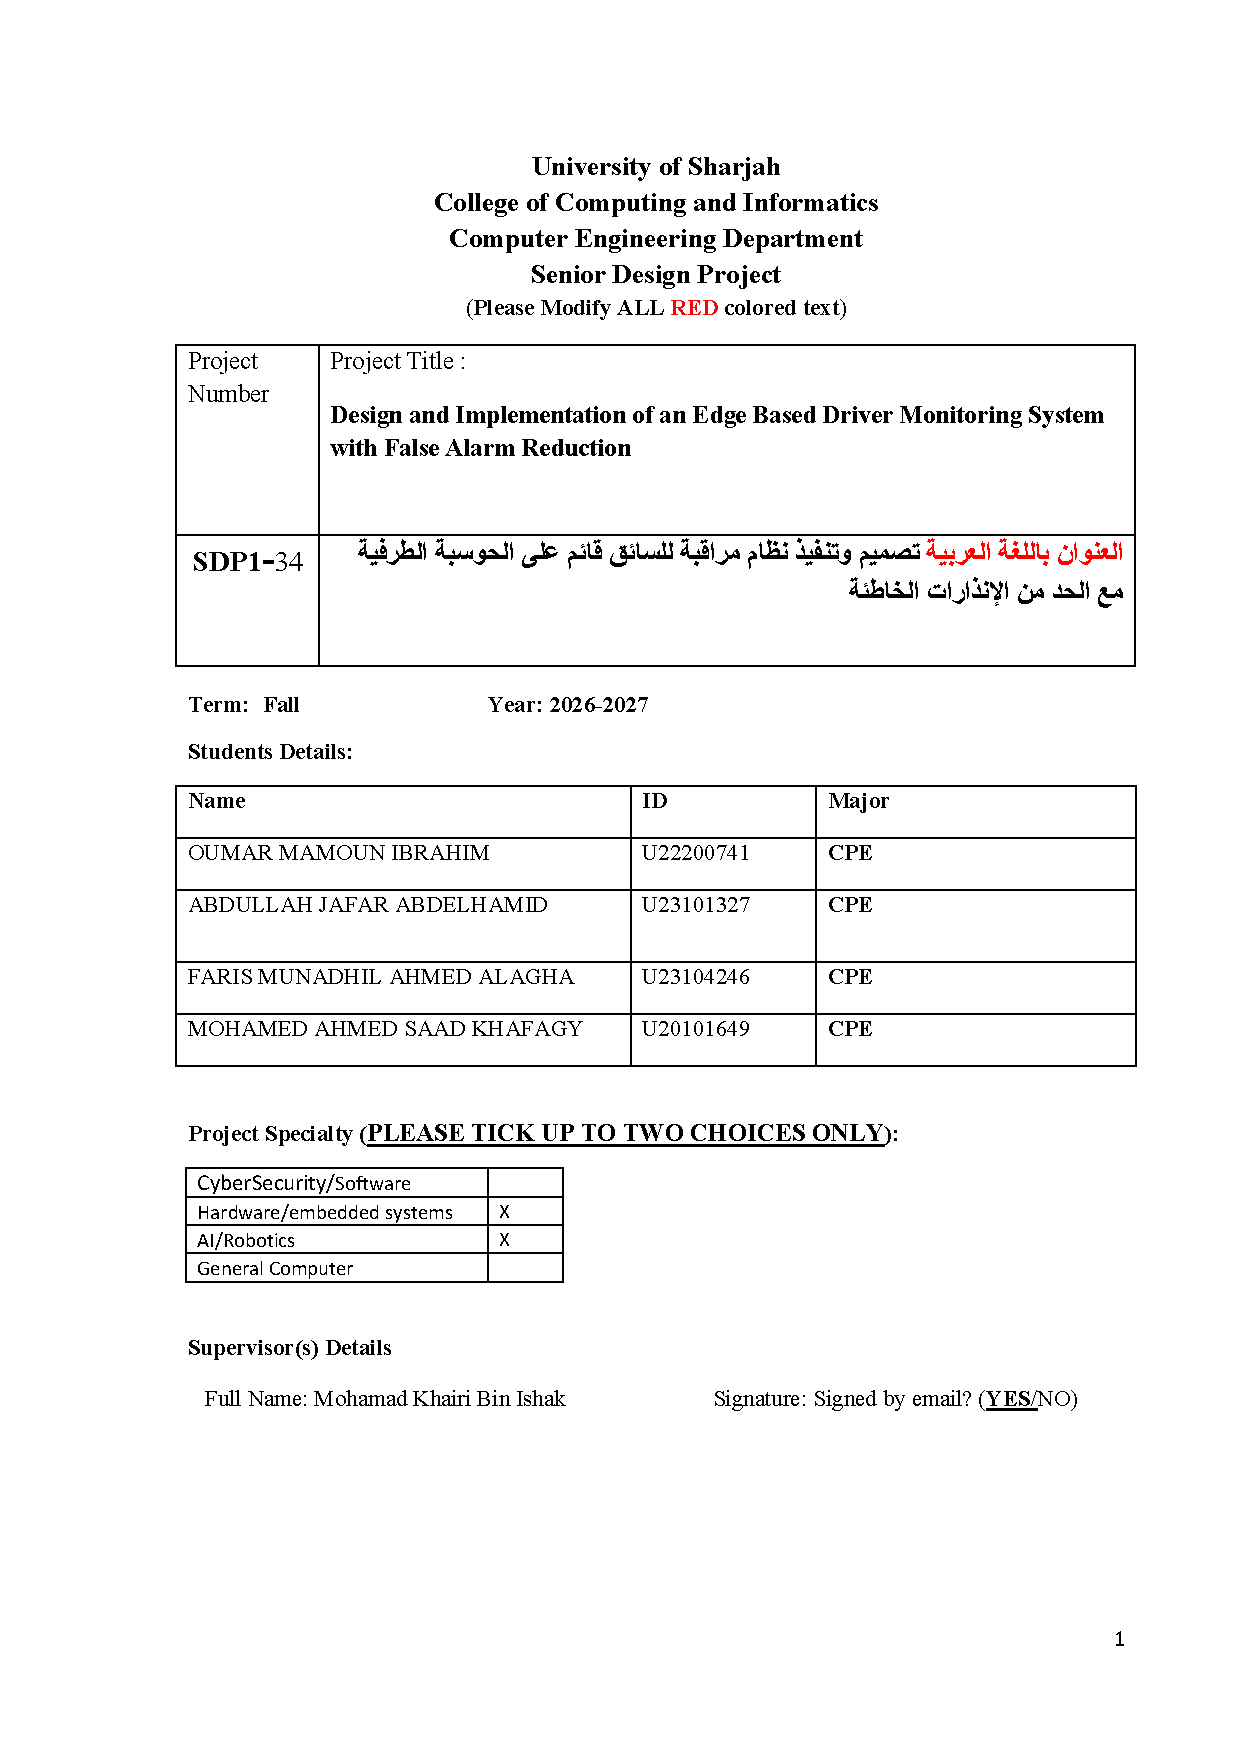
\includepdf[pages=-, scale=0.85, pagecommand={\thispagestyle{plain}}]{Template/SDP1_N34_Proposal.pdf}
